\documentclass{article}
\usepackage{graphicx} % Required for inserting images
\usepackage{float}
\usepackage[T1]{fontenc}
\usepackage{amsmath}
\usepackage[margin=1in]{geometry}
\usepackage{booktabs}
\usepackage{tabularx}
\usepackage[hidelinks]{hyperref}

\title{Signalling with HAR instead of GARCH on the short-only book}
\author{Experiment report \textperiodcentered{} L/S Gamma Desk, QUANTT}
\date{2026-10-16}

\begin{document}

\maketitle

\textbf{Question:} On the short-only book, does signalling with the HAR forecaster instead of GARCH raise net P\&L at 1x and 2x spreads, in both halves of the window, without a worse daily tail?

\textbf{Method:}

\begin{itemize}

\item \textbf{Pre-registration:} the hypothesis card was committed before any run (commit 671df4e).

\item \textbf{Data:} the live paper rules (\texttt{configs/\allowbreak{}paper.\allowbreak{}toml}) are replayed on R2 replay snapshots v1 (config\_hash b040760187f0) over the development window 2014-06-02 to 2024-12-31. Spot comes from put-call parity on the 30-minute grid (10:15 to 15:45 ET). The hold-out (2025-01-01 to 2026-07-10) was not used.

\item \textbf{Book:} short-only (\texttt{[signal] long\_\allowbreak{}band = -\allowbreak{}inf}), with the live short band of +0.02. That means a short put near 30 DTE, 1 contract, with the signal, exits and hedge at 10:15 ET.

\item \textbf{Forecast:} the live \texttt{runner.\allowbreak{}forecast} code with \texttt{FORECASTERS[``har'']}. It is fit on the last 5 years of daily SPY returns (completed days only) and forecasts vol over the chosen expiry's DTE. This HAR runs on squared daily returns: it is the same model that lost to GARCH on forecast error (QLIKE) in \texttt{2026-\allowbreak{}10-\allowbreak{}05-\allowbreak{}har-\allowbreak{}vs-\allowbreak{}garch}.

\item \textbf{Variants:}

\begin{itemize}

\item \texttt{har} (primary): \texttt{[signal] forecaster = ``har''}, \texttt{long\_\allowbreak{}band = -\allowbreak{}inf}.

\item \texttt{short\_\allowbreak{}only} (reference): the registered runs of \texttt{2026-\allowbreak{}10-\allowbreak{}16-\allowbreak{}short-\allowbreak{}only/\allowbreak{}short\_\allowbreak{}only} (GARCH). The config is identical except for the forecaster, and the runs were reused, not rerun.

\item The baseline (live rules, trial 1) is shown in the charts for context only.

\end{itemize}

\item \textbf{Runs:} \texttt{har} ran once at 1x and 2x spreads. Costs are \$0.65 per contract and \$0.005 per share, with a \$1 minimum per order.

\end{itemize}

This report was written by Claude at the PM's request.

\section{Result vs the pass bar}

\texttt{har} is compared with \texttt{short\_\allowbreak{}only} at the same spread multiple, and every check had to hold at both 1x and 2x. P\&L is net USD on daily equity for 1 contract. ES is the mean of the worst 5\% of daily P\&L.

\begin{center}\small
\begin{tabularx}{\linewidth}{>{\raggedright\arraybackslash}X l l l l l}
\toprule
\textbf{Check} & \textbf{1x value} & \textbf{1x bar} & \textbf{2x value} & \textbf{2x bar} & \textbf{Result} \\
\midrule
Net P\&L, full window & \ensuremath{-}1,250 & > \ensuremath{-}774 & \ensuremath{-}2,682 & > \ensuremath{-}2,351 & fail \\
Net P\&L, 2014-06 to 2019-12 & \ensuremath{-}854 & > \ensuremath{-}875 & \ensuremath{-}1,244 & > \ensuremath{-}1,261 & pass \\
Net P\&L, 2020-01 to 2024-12 & \ensuremath{-}396 & > +101 & \ensuremath{-}1,438 & > \ensuremath{-}1,090 & fail \\
abs ES 5\% \ensuremath{\leq} 1.10 \ensuremath{\times} reference & 87.4 & \ensuremath{\leq} 94.1 & 93.7 & \ensuremath{\leq} 101.7 & pass \\
Event floor: round trips (1x) & 86 & \ensuremath{\geq} 30 &  &  & met \\
\bottomrule
\end{tabularx}
\end{center}

\textbf{Verdict: failed.} HAR loses \$476 more than GARCH at 1x and \$331 more at 2x. The 2014-2019 half is a near-tie (\$21 and \$17 better). The whole shortfall is in 2020-2024, and the book loses money with either forecaster.

\subsection{Full-window numbers (not part of the bar)}

\begin{center}\small
\begin{tabularx}{\linewidth}{>{\raggedright\arraybackslash}X >{\raggedright\arraybackslash}X l >{\raggedright\arraybackslash}X l}
\toprule
\textbf{} & \textbf{short\_only 1x} & \textbf{har 1x} & \textbf{short\_only 2x} & \textbf{har 2x} \\
\midrule
Net P\&L & \ensuremath{-}774 & \ensuremath{-}1,250 & \ensuremath{-}2,351 & \ensuremath{-}2,682 \\
Round-trip P\&L before commissions & +318 & \ensuremath{-}281 & \ensuremath{-}1,240 & \ensuremath{-}1,696 \\
Sharpe on \$250k & \ensuremath{-}0.15 & \ensuremath{-}0.25 & \ensuremath{-}0.42 & \ensuremath{-}0.51 \\
Max drawdown & 2,220 & 2,559 & 3,222 & 3,445 \\
ES 5\% (daily) & \ensuremath{-}85.5 & \ensuremath{-}87.4 & \ensuremath{-}92.4 & \ensuremath{-}93.7 \\
Round trips & 100 & 86 & 100 & 86 \\
Win rate & 57\% & 59\% & 54\% & 56\% \\
Short-signal days & 466 & 423 & 466 & 423 \\
Commissions (options /\allowbreak{} hedges) & 200 /\allowbreak{} 770 & 172 /\allowbreak{} 678 & 200 /\allowbreak{} 770 & 172 /\allowbreak{} 678 \\
\bottomrule
\end{tabularx}
\end{center}

\section{Charts}

\begin{figure}[H]\centering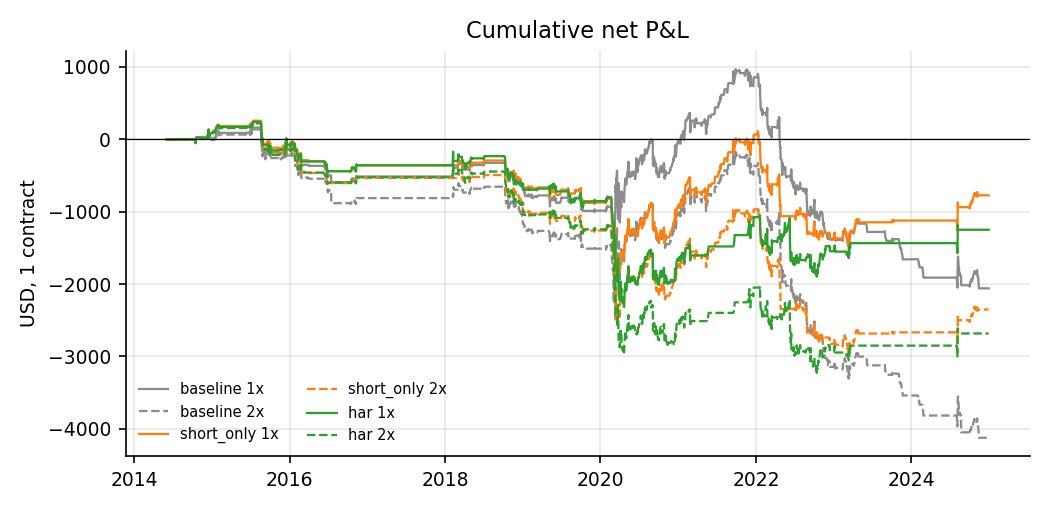
\includegraphics[width=0.92\linewidth]{figures/cum_pnl.png}\caption{Cumulative net P\&L, 1x solid and 2x dashed; baseline (live rules) grey}\end{figure}

The two short-only lines track each other until early 2020. In the March 2020 crash HAR drops further, and it then recovers less in 2020-2021. It claws back much of the gap in 2022, but it trails again in 2023-2024, when it hardly trades.

\begin{figure}[H]\centering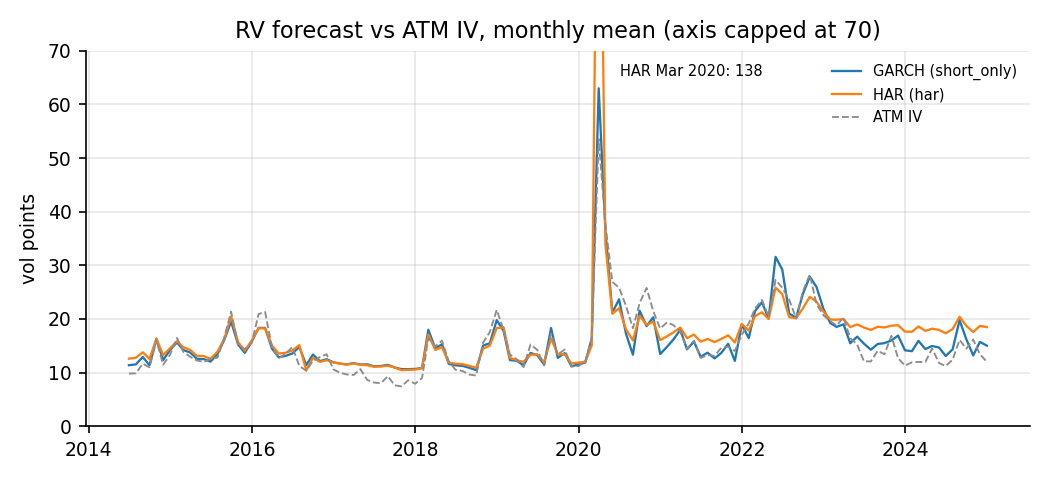
\includegraphics[width=0.92\linewidth]{figures/rv_forecast.png}\caption{RV forecast vs ATM IV, monthly mean}\end{figure}

Before 2020 the two forecasts are close. In March 2020 HAR's monthly mean reaches 138 vol points, against GARCH's 63. From 2021 on, HAR sits above GARCH in calm stretches: the median daily gap is +2.2 points in 2021, +2.7 in 2023 and +3.4 in 2024. In 2022 it sits below (\ensuremath{-}1.4). Over the whole window HAR's median forecast is 15.8 against 14.0 for GARCH, with a median ATM IV of 13.7.

\begin{figure}[H]\centering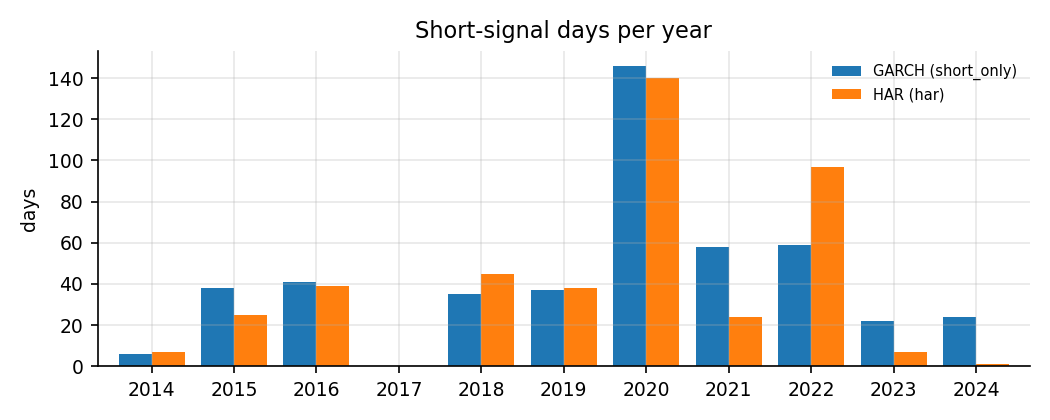
\includegraphics[width=0.92\linewidth]{figures/short_days.png}\caption{Short-signal days per year}\end{figure}

A higher forecast means a lower VRP, so fewer short days. HAR signals short on 423 days against 466. Of those days, 336 are shared, 130 are GARCH-only and 87 are HAR-only. The difference is concentrated after 2020:

\begin{center}\small
\begin{tabularx}{\linewidth}{>{\raggedright\arraybackslash}X l l l l}
\toprule
\textbf{Short-signal days} & \textbf{2021} & \textbf{2022} & \textbf{2023} & \textbf{2024} \\
\midrule
GARCH & 58 & 59 & 22 & 24 \\
HAR & 24 & 97 & 7 & 1 \\
\bottomrule
\end{tabularx}
\end{center}

In 2014-2019 the counts are nearly equal (154 against 157).

\begin{figure}[H]\centering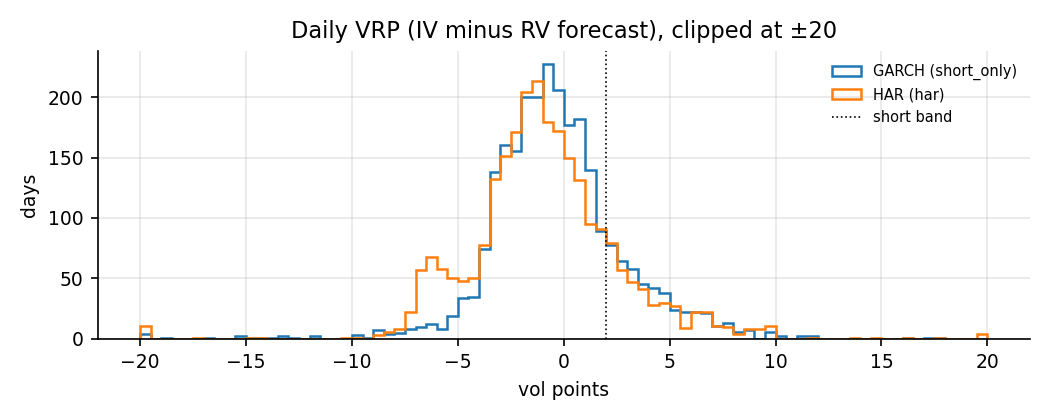
\includegraphics[width=0.92\linewidth]{figures/vrp_dist.png}\caption{Daily VRP (IV minus RV forecast)}\end{figure}

Above the short band (+2 points), the two VRP distributions are almost the same shape. The difference is a second hump in HAR's distribution between \ensuremath{-}7 and \ensuremath{-}5 points: days on which HAR's forecast sat well above IV and kept the book flat. The median VRP is \ensuremath{-}1.1 points for HAR and \ensuremath{-}0.6 for GARCH.

\begin{figure}[H]\centering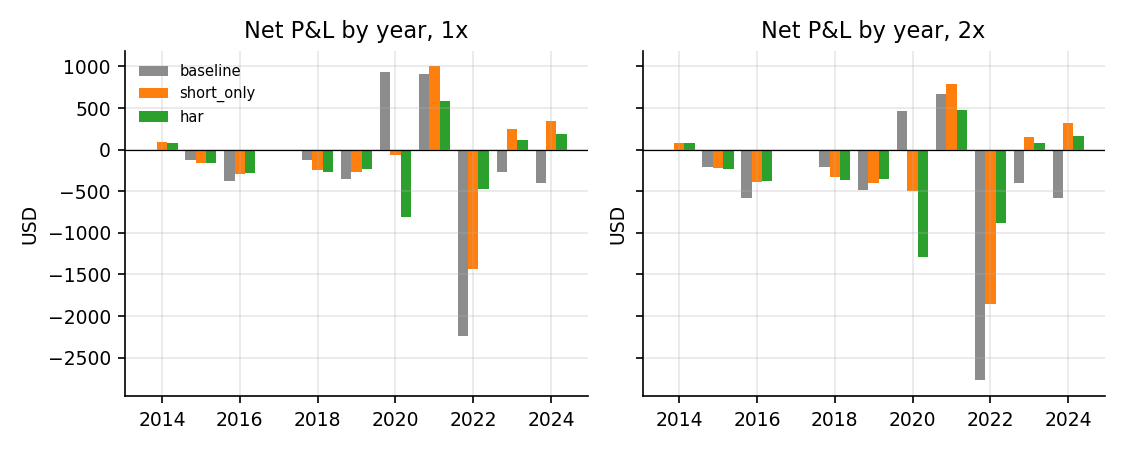
\includegraphics[width=0.92\linewidth]{figures/yearly.png}\caption{Net P\&L by year}\end{figure}

At 1x, HAR is better or level in 2014-2019 (+\$21 in total) and in 2022 (\ensuremath{-}\$470 against \ensuremath{-}\$1,433). It is worse in 2020 (\ensuremath{-}\$804 against \ensuremath{-}\$60), 2021 (+\$582 against +\$1,000), 2023 (+\$111 against +\$244) and 2024 (+\$185 against +\$349). The 2x pattern is the same.

\begin{figure}[H]\centering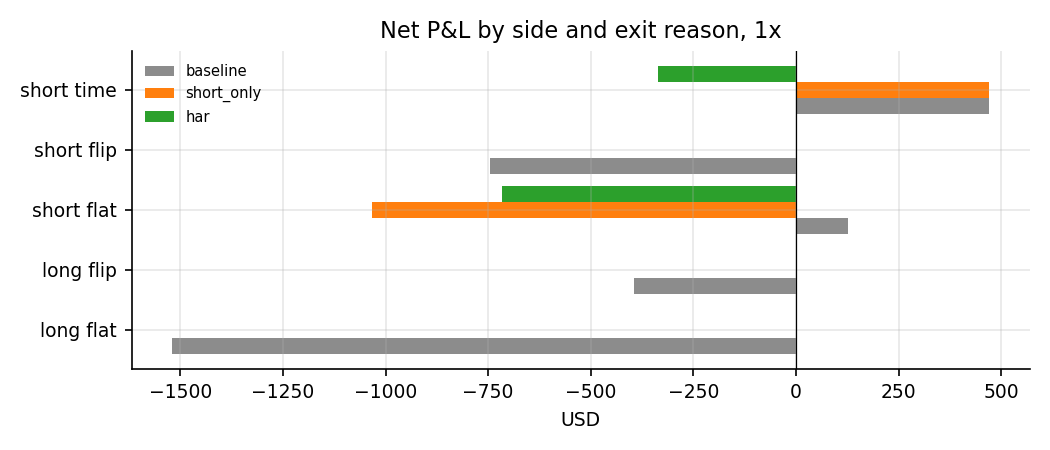
\includegraphics[width=0.92\linewidth]{figures/by_reason.png}\caption{Net P\&L by side and exit reason, 1x}\end{figure}

The two books close a similar number of shorts at the time exit (13 each), but HAR's time exits lose \$336 net, while GARCH's make \$470. Four of HAR's time exits came in 2022 and lost \$670 together. HAR's flat exits lose less in total (\ensuremath{-}\$716 from 73, against \ensuremath{-}\$1,032 from 87), mostly because there are fewer of them.

\begin{figure}[H]\centering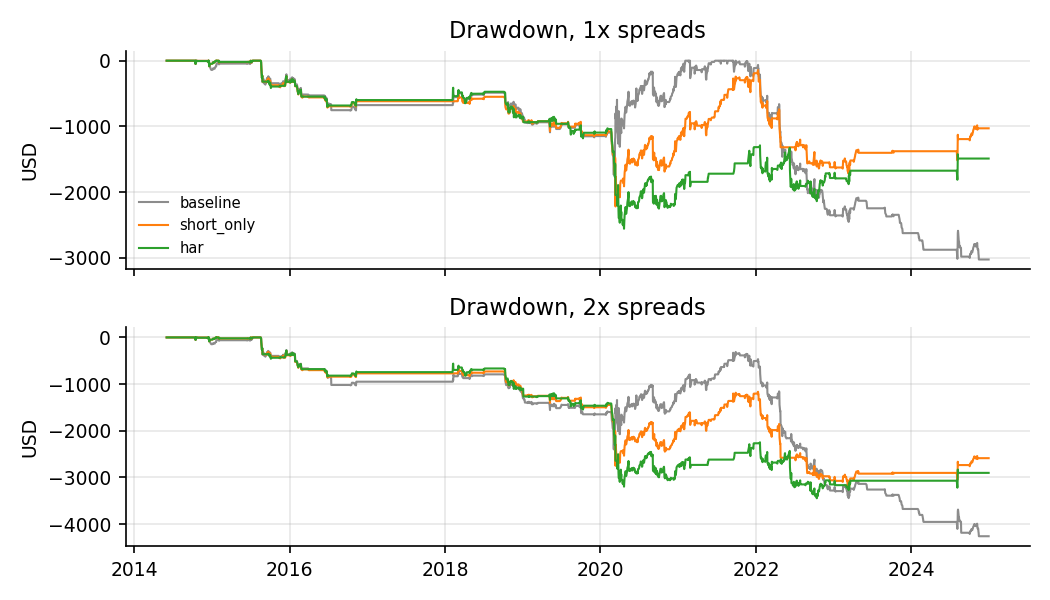
\includegraphics[width=0.92\linewidth]{figures/drawdown.png}\caption{Drawdown at 1x and 2x spreads}\end{figure}

HAR's drawdown is deeper from March 2020 through 2021, and its maximum drawdown is larger at both multiples (1x \$2,559 against \$2,220; 2x \$3,445 against \$3,222). The daily ES is within the 1.10x guard at both.

\begin{figure}[H]\centering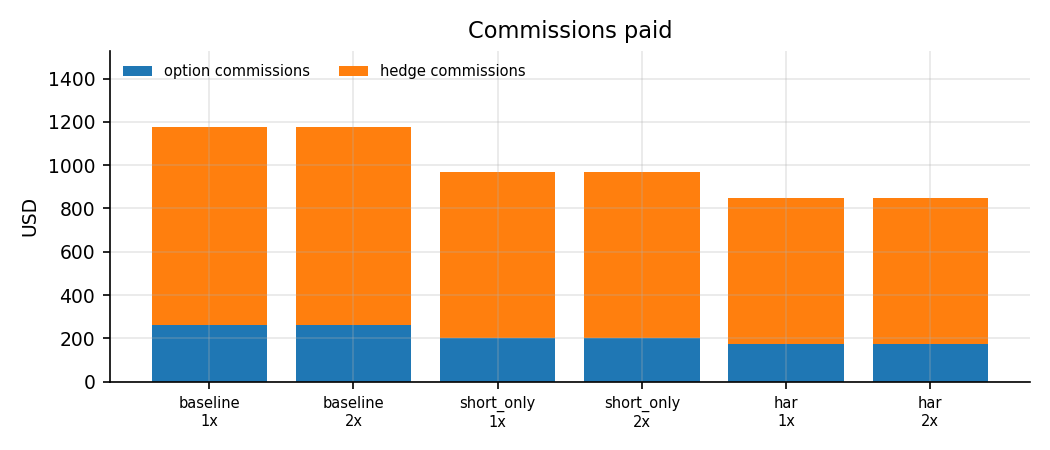
\includegraphics[width=0.92\linewidth]{figures/fees.png}\caption{Commissions paid}\end{figure}

Fewer round trips mean slightly lower commissions: \$850 against \$970 at both multiples. The saving is small next to the P\&L gap.

\section{Analysis}

\textbf{The P\&L bridge.} The change from \texttt{short\_\allowbreak{}only} to \texttt{har}, at 1x and 2x:

\begin{center}\small
\begin{tabularx}{\linewidth}{>{\raggedright\arraybackslash}X l l}
\toprule
\textbf{} & \textbf{1x} & \textbf{2x} \\
\midrule
Round-trip P\&L before commissions & \ensuremath{-}\$598 & \ensuremath{-}\$456 \\
Commissions attributed to round trips & +\$108 & +\$108 \\
Unattributed unwind residual & +\$15 & +\$17 \\
Change in net P\&L & \ensuremath{-}\$476 & \ensuremath{-}\$331 \\
\bottomrule
\end{tabularx}
\end{center}

The unwind residual is equity P\&L minus the round-trip net P\&L. It is almost the same in both books (about \ensuremath{-}\$200), so hedge-unwind fill noise does not drive this result. The loss is in the trades themselves.

\textbf{Matched and unmatched trades (1x).}

\begin{itemize}

\item \textbf{Matched:} 41 of the entries fall on the same day in both books, and 33 of those also close on the same day. On these matched entries HAR does \$410 better (\ensuremath{-}\$944 against \ensuremath{-}\$1,355). 2022 (+\$820) more than accounts for it, where HAR's signal stayed short longer and changed the exits. 2020 goes the other way (\ensuremath{-}\$303).

\item \textbf{Unmatched:} the trades only one book took decide the result. GARCH's 59 unmatched trades made +\$793, and HAR's 45 made \ensuremath{-}\$108. The GARCH-only trades that made money were mostly shorts after the crash: +\$1,167 from 8 in 2020, plus +\$378 in 2021 and +\$318 in 2023-2024. HAR was flat on those days because its forecast was above IV.

\item \textbf{Path dependence:} with one position at a time, a different entry shifts every later entry, so the matched/\allowbreak{}unmatched split is approximate.

\item At 2x the split is the same: matched +\$547, unmatched \ensuremath{-}\$895.

\end{itemize}

\textbf{Three separate effects, which mostly do not offset.}

\begin{enumerate}

\item \textbf{Calm years after a shock (2021, 2023-2024).} HAR's five-year fit window contains the 2020 crash, and its forecast stayed 2-3 points above GARCH's. This matches the earlier QLIKE finding that our HAR stays elevated after shocks. On this book that switched off most of the calm-year premium (2024: 1 short day against 24), costing \$715 at 1x over those three years.

\item \textbf{The 2020 crash.} In early March HAR lagged: its median forecast was 35, against 40 for GARCH and 43 for IV. In the second half of March it was unstable, ranging from its variance floor (near 0\%, on one day) up to 777\%. The fit uses squared daily returns with nothing to keep the forecast positive except a floor. HAR still signalled short on 3 days in late March, when GARCH signalled none. The two shorts HAR opened in March 2020 lost \$1,046 together, against +\$28 for GARCH's one March short. HAR's 2020 is \$744 worse at 1x.

\item \textbf{2022.} HAR's forecast sat below GARCH's. It traded more and lost \$963 less at 1x, mostly through the exit timing of matched trades. This is the one place HAR helps, and it depends on a handful of trades and their path.

\end{enumerate}

Excluding 2022, HAR would trail by about \$1,440 at 1x. So HAR is not picking better short days. It mostly keeps the book flat in calm years and sells at the wrong time in a crash. The pre-2020 near-tie shows the two forecasters agree when there is no recent shock in the fit window.

\section{Verdict}

\textbf{Failed} on the pre-registered bar: the full window and the 2020-2024 half fail at both 1x and 2x. ES stays within the guard, and the event floor is met (86 round trips). Keep GARCH as the live forecaster and archive this test.

\textbf{Possible follow-up} (it would need its own card and is in-sample): the HAR variant suggested in \texttt{2026-\allowbreak{}10-\allowbreak{}05-\allowbreak{}har-\allowbreak{}vs-\allowbreak{}garch}, fit on Garman-Klass or intraday realized variance instead of squared returns. A positivity guard on the forecast should come first. The March 2020 behaviour shows the current HAR can produce forecasts far outside any plausible range.

\section{Caveats}

\begin{itemize}

\item \textbf{In-sample:} the idea comes from the 2026-10-16 desk discussion of the baseline on this same window.

\item \textbf{Which HAR:} this tests the desk's HAR on squared daily returns, not HAR as designed (on intraday realized variance). The result does not rule out a better-built HAR.

\item \textbf{Path dependence:} with one position at a time, a changed entry or exit shifts every later trade. The 2022 gain and the 2020 loss each rest on a few trades.

\item \textbf{One contract:} the \$1 minimum per order is large relative to size.

\item \textbf{Spread model:} fitted on about two weeks of calm 2026 live quotes. The 2x run is the stress test.

\item \textbf{Data gaps:} R2 has no month-end weekdays, so 89 scheduled times (3.3\%) are skipped in both books.

\item \textbf{Few events:} 36 round trips in 2014-2019 and 50 in 2020-2024 for \texttt{har}.

\end{itemize}

\section{Trials}

There are 2 trials for this experiment (\texttt{har} at 1x and 2x, one run of \texttt{experiment.\allowbreak{}py}, commit 671df4e, no \texttt{-\allowbreak{}dirty} tag), plus the baseline's 2. The reference was reused from \texttt{2026-\allowbreak{}10-\allowbreak{}16-\allowbreak{}short-\allowbreak{}only} (2 trials, not rerun). After the run, one chart was changed: the forecast chart's y-axis is now capped at 70 with the March 2020 peak labelled, because the uncapped peak flattened every other month. The figures were rebuilt with \texttt{-\allowbreak{}-\allowbreak{}report-\allowbreak{}only}, which adds no trials. The pass bar was not changed.

\end{document}
